\documentclass{ctexart} %%%编译方式 XeLaTeX

 %\usepackage{amsthm}
\title{分解定理}

\author{时侠圣(11710009)}

\begin{document}
\maketitle

\section{背景}
多说站在食物链顶端的动物们,例如狮子、老虎等主要靠视觉来搜寻猎物,和靠气味觅食(大白鲨)不同,视觉不存在所谓的梯度差,看不见就是看不见,没有动物具有透视眼。所以觅食策略对于狮子老虎这样的陆地动物是很重要的。在不知道猎物位置的情况下,\textcolor{red}{布朗运动}或许是最自然的方法了。布朗运动是一个随机过程,它的步长服从\textcolor{red}{正态分布}。离散版的布朗运动叫做\textcolor{red}{随机游走}(Random walk),它的步长和方向都是离散的。尽管布朗运动和随机游走是两个概念,也各自发展出了一套不同的理论,但两者的数学本质是一样的。如下布朗运动的轨迹图。

\begin{figure}[hbt!]
  \centering
  % Requires \usepackage{graphicx}
  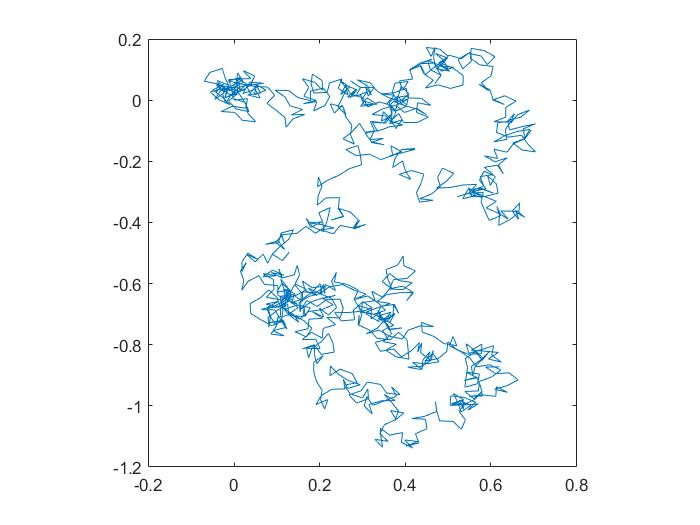
\includegraphics[width=8cm]{5/figure/14.jpg}\\
  \caption{布朗运动轨迹图}\label{fig14}
\end{figure}


在物理学家眼里,布朗运动可以用\textcolor{red}{郎之万方程}来描述:
\begin{equation}
m\frac{d^2x}{dt^2}=f(t)+F^{'}(t).
\end{equation}
其中$f(t)$分成两部分,一部分为阻力$-\alpha v$; 一部分为随机作用力$F(t)$。 粘滞阻力仍来自介质分子对颗粒的碰撞,将颗粒看作半径为$a$的小球,在粘滞系数为$\eta$ 的流体中运动,则有$\alpha=6\pi\eta a$。
\begin{equation}
m\ddot{x}=-\mu \dot{x}(t)+\eta(t).
\end{equation}
其中$\eta(t)$是均值为0,方差为常数的随机过程。更确切地讲,是白噪声过程。

因此郎之万方程本质上就是考虑了\textcolor{red}{随机误差}的牛顿第二定律,这样的方程又叫做\textcolor{red}{随机微分方程}(Stochastic Differential Equation)。尽管郎之万是第一个提出随机过程的人,但作为物理学家,他更关心这些方程是否符合实际物理现象,而不关心数学上的严谨性。因此这种模型并没有立即受到数据家的重视。

到了二十世纪中叶,日本数学家伊藤清和苏联数学家Stratonovich先后使用概率论的方法,把随机微分方程发展成严谨的数学概念。尽管如此,但两人对随机微分方程定义各有不同,这也显示了\textcolor{red}{随机性}和\textcolor{red}{确定性}的本质差异。此外,随机微分方程多用于对一些多样化现象进行建模,比如不停变动的股票价格、部分物理现象如热扰动等。

如果捕食者像无头苍蝇一样漫无目的的做布朗运动,真的能很有效的地寻到到猎物吗?在数学上可以证明,布朗运动和分子自由扩散一样,单位速度的分子在时间$t$ 内平均只有$\sqrt{t}$的位移量。捕食者若采用此种策略,可能需要踏遍千山万水才能成功了。

那么有没有比布朗运动更高效的搜索方法呢?一组巴西物理学家于1999年提出了一个设想,认为“莱维飞行”比布朗运动有更高的搜索效率,因此自然会偏向与采用“莱维飞行”捕食的生物。
\section{莱维分布}
 莱维分布(Levy Distribution)是由P.Levy 在19世纪30年代提出的一类分布,这种分布有两个参数:$\alpha$和$\gamma$。参数$\gamma>0$,参数$\alpha$用于控制分布的形状,且满足$0<\alpha\le2$。事实上当$\gamma=1$时,莱维分布就转换为柯西分布,而当$\gamma=2$时,莱维分布则为正态分布。莱维分布的概率密度函数为
  \begin{equation}
  L_{\alpha,\gamma}=\frac{1}{\pi}\int_0^{\infty}e^{-\gamma q^{\alpha}}cos(qy)dq,y\in\mathcal{R}.
  \end{equation}
 上述积分很难积,因此现有的莱维分布基本上使用数值方法计算。设$x,y$ 是两个独立同分布的随机变量,且均为标准正态分布,令随机变量$v$满足:
 \begin{equation}
 v=\frac{x}{\sqrt{y}}
 \end{equation}
 则随机变量$\{z_n\}_{n=1}^{+\infty}$为
 \begin{equation}
 z_n=\frac{1}{\alpha\sqrt{n}}\sum_{j=1}^nv_j
 \end{equation}
 在概率论中,我们可以用特征函数来描述一个随机变量。此时,我们有如下重要定理。

 \textbf{定理1}(莱维-辛钦公式):
莱维过程$\{X(t),t\ge0\}$的特征函数(傅里叶变换)表达如下:
\begin{equation}
\phi_X(\theta)(t):=E[e^{i\theta X(t)}]=\exp(t(ai\theta-\frac{1}{2}\sigma^2\theta^2+\int_{\mathcal{R} \backslash \{0\}}(e^{i\theta x}-1-i\theta xI_{|x|<1})\prod(dx))).
\end{equation}
这个定理的证明比较复杂,依赖于测度论中的一系列结果。
 收敛于莱维分布。现在提供一个matlab例子。轨迹如下:
\begin{figure}[hbt!]
  \centering
  % Requires \usepackage{graphicx}
  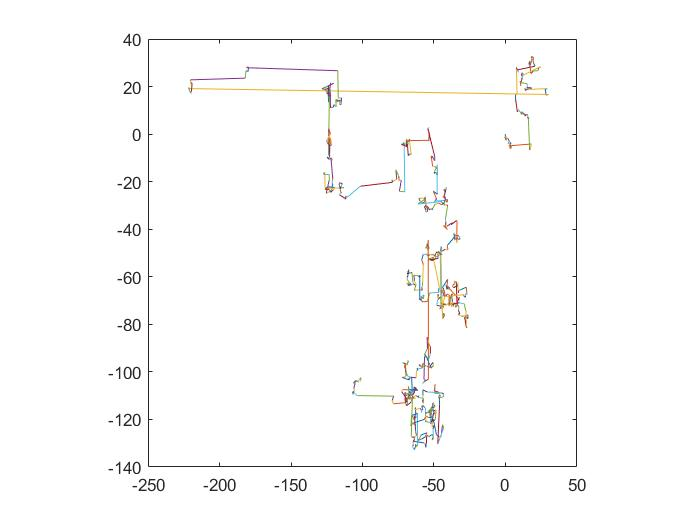
\includegraphics[width=8cm]{5/figure/13.jpg}\\
  \caption{Levy分布轨迹图}\label{fig13}
\end{figure}
随机变量$X$是无限可分的,除非它的该率分布$p_x$是无限可分的,例如,$X=Y_1^{(n)}+...+Y_n^{(n)}$,其中$Y_1^{(n)},...,Y_n^{(n)}$是独立同分布。那么$X$的特征函数可以写成$\Phi_X(u)=(\Phi_{Y_1^{(n)}}(u))^n$。莱维过程$\{X(t),t\ge0\}$是一种随机过程,它满足的条件比布朗运动宽松:

 1.$X(0)$ 几乎处处为0;

 2.独立增量性;

 3.稳定增量性;

 4.样本轨道右连续。

连续的布朗运动和离散的泊松过程都是莱维过程的特例。因此可以大胆猜测,莱维过程就是带“跳跃”的布朗运动。正是这些不连续性 的“跳跃”给予莱维过程“重尾”的特性。

 \textbf{独立增量:}设$X(t)$是一个连续时间上的随机过程。也就是说,对于任何固定的$t\ge0$,$X(t)$是一个随机变量。过程的增量为差值$X(s)-X(t)$。独立增量意味着对于任意时间$s>t>u>v,X(s)-X(t)$与$X(u)-X(v)$相互独立。

 \textbf{稳定增量:} 如果增量$X(s)-X(t)$的分布只依赖于时间间隔$s-t$,则称增量是稳定的。例如对于维纳过程,增量$X(s)-X(t)$服从均值为0,方差为$s-t$的正态分布。对于泊松过程,增量$X(s)-X(t)$服从指数为$s-t$的泊松分布。
\section{分解定理}
 在给出莱维-伊藤分解定理之前,我们给出如下定义和推论。

\textbf{定义1:}
 莱维可测是满足如下条件的$\mathbf{R}^d\backslash\{0\}$上的测度$v$, 使得
 \begin{equation}
 \int(|y|^2\wedge1)v(dy)<\infty.
 \end{equation}
 其中$|y|^2\wedge1=\left\{\begin{array}{cc}1,&|x|>1\\
                                           y^2,&|x|\le1\end{array}\right.$

 定义函数$X:\mathbf{R}^{+}\to\mathbf{R}$ 是Cadlag 过程,即$X$ 是右连续左极限存在。令$\Delta X(t)=X(t)-X(t-)$(由于左极限的存在)且定义如下泊松随机测度
 \begin{equation}
 N(t,A)=\sharp \{\Delta X(s)\in A:s\in[0,t]\}.
 \end{equation}
 那么有如下结论:

 (1)$N(1,B_{\varepsilon}^c(0))<\infty$.

 (2)$N(1,\mathbf{R}\backslash \{0\})$是可数的。

 令$A$是有下界的,i.e., $0\not\in\overline{A}$.那么$N(t,A),t\ge0$是泊松过程且强度为$\mu(A)=\mathbf{E}[N(1,A)]$.很明显有结论$\mu(A)<\infty$不管$A$ 是否有下界。所以测度$\mu$是$\sigma-$有限的。

 \textbf{推论1:}
(1)对任意的$t>0,\omega\in\Omega,N(t,\cdot)(\omega)$ 在$\mathcal{B}(\mathbf{R}^d\backslash \{0\})$上是计数可测的。

(2)对于任意的有下界的$A$,$N(t,A),t\ge0$ 是泊松过程且具有如下强度$\mu(A)=\mathbf{E}[N(1,A)]$.

(3)补$\tilde{N}(t,A)=N(t,A)-t\mu(A)$是值鞅可测的。对于有下界的$A$, $\tilde{N}(t,A)$是一个鞅。

令$f:\mathbf{R}^d\to\mathbf{R}$是波莱尔可测函数,$A$有下界,那么对任意$t>0,\omega\in\Omega$,我们定义如下关于$f$泊松积分通过一个随机有限和。
\begin{equation}
\int_{A}f(x)N(t,dx)(\omega)=\sum_{x\in A}f(x)N(t,\{x\})(\omega).
\end{equation}






\textbf{定理2:}令$A$有下界,则

(1)对任意的$\int_{A}f(x)N(t,dx),t\ge0$是复合泊松过程,带有如下特征函数:
\begin{equation}
\mathbf{E}[exp\{iu\cdot\int_{A}f(x)N(t,dx)\}]=exp\{t\int_{A}(e^{iu\cdot x}-1)\mu_f(dx)\}.
\end{equation}
其中$u\in\mathbf{R}^d,\mu_f=\mu\circ f^{-1}$.

(2)如果有$f\in L^1(A,\mu_A)$,那么有
\begin{equation}
\mathbf{E}[\int_{A}f(x)N(t,dx)]=t\int_{A}f(x)\mu(dx).
\end{equation}

(3)如果有$f\in L^2(A,\mu_A)$,那么有
\begin{equation}
Var[|\int_{A}f(x)N(t,dx)|]=t\int_{A}|f(x)|^2\mu(dx).
\end{equation}

从定理2可以看出,如果$f\in L^1(A,\mu_A)$,一个泊松积分也许不一定全都有有限期望。对于此,我们定义如下补泊松积分:
\begin{equation}
\int_{A}f(x)\tilde{N}(t,dx)=\int_{A}f(x)N(t,dx)-t\int_{A}f(x)\mu(dx).
\end{equation}
则有如下结论:

(1) $\int_{A}f(x)\tilde{N}(t,dx),t\ge0$ 是一个鞅。

(2)
特征函数:
\begin{equation}
\mathbf{E}[exp\{iu\cdot\int_{A}f(x)\tilde{N}(t,dx)\}]=exp\{t\int_{A}(e^{iu\cdot x}-1-iu\cdot x)\mu_f(dx)\}.
\end{equation}
其中$u\in\mathbf{R}^d,\mu_f=\mu\circ f^{-1}$.


(3)如果有$f\in L^2(A,\mu_A)$,那么有
\begin{equation}
Var[|\int_{A}f(x)\tilde{N}(t,dx)|]=t\int_{A}|f(x)|^2\mu(dx).
\end{equation}

对于有下界的$A$和任意的$t>0$,$\int_{A}xN(t,dx)\sum_{0\le u\le t}\Delta X(u)1_A(\Delta X(u))$是集合$A$ 中不超过时间$t$的所有跳变值和。由于轨迹$X$ 是Cadlag, 所以上述是个有限随机和。特别地,$\int_{|x|\ge1}xN(t,dx)$is所有大于1的跳变之和。也就是说是一个带有有限次扰动的复合泊松过程。相反地,也可以证明$X(t)-\int_{|x|\ge1}xN(t,dx)$带有有限次有次序动作的莱维过程。但是也许有无界扰动。所以我们可以定义
 \begin{equation}
 b=\mathbf{E}[X(1)-\int_{|x|\ge1}xN(1,dx)].
 \end{equation}

 现在把关注度放在小跳变上来。引入$M(t,A)=\int_{A}f(x)\tilde{N}(t,dx)$.令$A_m=\{x:\frac{1}{m+1}<|x|\le1\}$.可以证明在$L^2$里,当$m\to\infty$ 时,我们有$M(t,A_m)\to\int_{|x|<1}x\tilde{N}(t,dx)$。 所以$\int_{|x|<1}x\tilde{N}(t,dx)$是一个鞅。取极限得
 \begin{equation}
\mathbf{E}[exp\{iu\cdot\int_{A}x\tilde{N}(t,dx)\}]=exp\{t\int_{A}(e^{iu\cdot x}-1-iu\cdot x)\mu(dx)\}.
\end{equation}
最后考虑如下随机过程
 \begin{equation}
W_{A}(t)=X(t)-bt-\int_{|x|<1}x\tilde{N}(t,dx)-\int_{|x|\ge1}xN(t,dx).
\end{equation}
那么随机过程$W_A(t)$是带有连续采样路径的中心鞅。利用布朗运动的莱维特征化,我们有$W_A(t)$就是协方差为$A$的布朗运动。

$X$是莱维过程。那么存在$b\in\mathbf{R}^d$, 协方差为$A$的布朗运动$W_A(t)$,$\mathbf{R}^{+}\times\{\mathbf{R}^d\backslash \{0\}\}$ 独立的泊松随机测度$N$使得下式成立:
\begin{equation}
X(t)=bt+W_{A}(t)+\int_{|x|<1}x\tilde{N}(t,dx)+\int_{|x|\ge1}xN(t,dx).
\end{equation}
其中平方可积鞅($L^2$-鞅)$\int_{|x|<1}x\tilde{N}(t,dx)$是所有小跳变的补和。上述跳变是以1为界的,可以推广至任意实数$R>0$,我们有
\begin{equation}
X(t)=b_Rt+W_{A}(t)+\int_{|x|<R}x\tilde{N}(t,dx)+\int_{|x|\ge R}xN(t,dx).
\end{equation}
其中$b_R=\mathbf{E}[X(1)-\int_{|x|\ge R}xN(1,dx)]$.可以计算如下:

(1)如果$1<R<\infty$,有$b_R=b+\int_{1\le|x|x<R}x\mu(dx).$

(2)如果$0<R<1$,有$b_R=b-\int_{R\le|x|x<1}x\mu(dx).$

是否可以去除上届约束$R$呢?此时我们有
\begin{equation}
X(t)=b_{\infty}t+W_{A}(t)+\int_{|x|\ge 0}x\tilde{N}(t,dx).
\end{equation}
结论是可以的,如果我们有$\mathbf{E}[X(1)]<\infty$。此时,我们有$b_{\infty}=\textbf{E}[X(1)]<\infty$.

同时,我们也可用通俗的语言表述上述定理。

\textbf{定理2}(莱维-伊藤分解):
每个莱维过程$\{X(t),t\ge0\}$都可以分解为$\{S(t),t\ge0\}$,$\{Y(t),t\ge0\}$ 和$\{Z(t),t\ge0\}$三个子过程,其中:

1.$S(t)$ 是维纳过程(就是布朗运动,莱维过程的连续部分);

2.$Y(t)$ 是复合泊松过程(刻画了较极端的“跳跃”现象);

3.$Z(t)$ 是平方可积的离散鞅(刻画了较小的“跳跃”现象)。

% 随机变量$(r.v.)X\sim\mu$的特征函数是映射$\Phi:\mathbf{R}^{d}\to\mathbf{C}$,定义如下
%% \end{document}
% \begin{equation}
% \Phi(u)=\mathbf{E}(e^{iu\cdot X})=\int_{R^d}e^{iu\cdot y}\mu(dy).
% \end{equation}
\end{document}
